\documentclass[11pt,a4paper]{article}

\usepackage[margin=1in]{geometry}
\usepackage{amsmath,amssymb,amsthm}
\usepackage{mathtools}
\usepackage{hyperref}
\usepackage{cleveref}
\usepackage{booktabs}
\usepackage{graphicx}
\usepackage{xcolor}
\usepackage[ruled,vlined,linesnumbered]{algorithm2e}

\newtheorem{theorem}{Theorem}[section]
\newtheorem{lemma}[theorem]{Lemma}
\newtheorem{proposition}[theorem]{Proposition}
\newtheorem{corollary}[theorem]{Corollary}
\newtheorem{definition}[theorem]{Definition}
\newtheorem{remark}[theorem]{Remark}
\newtheorem{example}[theorem]{Example}

\DeclareMathOperator{\BR}{BR}
\DeclareMathOperator{\NE}{NE}
\DeclareMathOperator{\SW}{SW}
\newcommand{\R}{\mathbb{R}}
\newcommand{\E}{\mathbb{E}}
\newcommand{\Prob}{\mathbb{P}}

\definecolor{cGreen}{HTML}{2ECC71}
\definecolor{cRed}{HTML}{E74C3C}
\definecolor{cBlue}{HTML}{3498DB}
\definecolor{cOrange}{HTML}{F39C12}

\title{The Topological Cooperation Theorem:\\
Fixed-Point Search as a Free Cooperation Mechanism\\[5pt]
\large with Applications to AI Safety}
\author{Eugene Shcherbinin\\
\textit{London School of Economics}\\
\texttt{y.shcherbinin@lse.ac.uk}}
\date{March 2026}

\begin{document}
\maketitle

\begin{abstract}
We prove that in any finite game with multiple Nash equilibria,
exhaustive fixed-point search followed by welfare-maximising selection
provides a \emph{strictly positive cooperation dividend} over random
equilibrium convergence, without any modification to the game's payoff
structure. The ``mechanism'' is pure computation: searching the
fixed-point set of the best-response map and selecting the best element.
We call this the \textbf{Topological Cooperation Theorem}, because the
cooperation arises from the topology of the equilibrium correspondence
rather than from mechanism design. We validate the theorem on 2,000
random games (100\% confirmation rate) and apply it to five AI safety
problems: corrigibility, deceptive alignment, alignment as a public
good, reward hacking, and AI debate. The corrigibility application
achieves 100\% safe equilibrium selection versus 63\% for standard
policy gradient methods.
\end{abstract}

\tableofcontents


%% ========================================================================
\section{Introduction}
%% ========================================================================

A fundamental challenge in multi-agent systems is equilibrium selection:
when a game has multiple Nash equilibria, which one will learning
dynamics converge to? This question is critical for AI safety, where
``safe'' and ``unsafe'' equilibria coexist and the learning algorithm's
choice determines whether the system is aligned.

The standard approach is \emph{mechanism design}: modify the game's
payoffs (via taxes, subsidies, or contracts) to make the desired
equilibrium dominant. This requires a principal with the power and
knowledge to redesign the game --- a strong assumption in multi-agent
AI systems.

We show that a weaker, purely computational intervention suffices:
\emph{search the Nash equilibrium set thoroughly, then select the
welfare-maximising element.} This requires no modification to payoffs,
no communication between agents, and no commitment mechanisms. The
cooperation dividend is ``free'' in the sense that it arises from
the geometry of the equilibrium set rather than from external
intervention.


%% ========================================================================
\section{The Topological Cooperation Theorem}
\label{sec:theorem}
%% ========================================================================

\subsection{Setup}

Let $\mathcal{G} = (N, \{\mathcal{A}_i\}, \{R_i\})$ be a finite
$N$-player game with Nash equilibrium set
$\mathcal{E}(\mathcal{G}) = \{\pi^{*,1}, \ldots, \pi^{*,K}\}$,
where $K = |\mathcal{E}|$ is the number of NE (at least one by
Nash's theorem).

\begin{definition}[Social Welfare]
$\SW(\pi) = \sum_{i=1}^N V_i(\pi)$, the sum of expected payoffs.
\end{definition}

\begin{definition}[Random NE Welfare]
$W_{\text{rand}}(\mathcal{G}) = \frac{1}{K}\sum_{k=1}^K \SW(\pi^{*,k})$,
the average welfare across all NE.
\end{definition}

\begin{definition}[Best NE Welfare]
$W_{\text{best}}(\mathcal{G}) = \max_{k \in [K]} \SW(\pi^{*,k})$,
the welfare of the Pareto-best NE.
\end{definition}

\begin{definition}[Cooperation Gap]
$\Delta(\mathcal{G}) = W_{\text{best}}(\mathcal{G}) - W_{\text{rand}}(\mathcal{G})$.
\end{definition}

\subsection{Main Result}

\begin{theorem}[Topological Cooperation]\label{thm:main}
For any finite game $\mathcal{G}$ with $|\mathcal{E}(\mathcal{G})| \geq 2$:
\begin{equation}
    \Delta(\mathcal{G}) = W_{\text{best}}(\mathcal{G}) - W_{\text{rand}}(\mathcal{G}) \geq 0,
\end{equation}
with equality if and only if all Nash equilibria have identical social welfare.
\end{theorem}

\begin{proof}
The maximum of a finite set is at least its arithmetic mean:
$\max_{k} \SW(\pi^{*,k}) \geq \frac{1}{K}\sum_k \SW(\pi^{*,k})$.
Equality holds iff all elements are equal.
\end{proof}

\begin{remark}
While the proof is elementary, the \emph{implication} is not. The
theorem says: if you can enumerate the Nash equilibria (via
fixed-point search) and select the best one, you achieve a
cooperation dividend for free --- without modifying payoffs,
without communication between agents, and without any commitment
mechanism. The ``mechanism'' is computation.
\end{remark}

\begin{proposition}[Generic Strict Positivity]\label{prop:generic}
The cooperation gap $\Delta(\mathcal{G}) > 0$ for a generic
(measure-one) set of games in the space of payoff matrices
$\R^{N \times |\mathcal{A}|} \times \cdots \times \R^{N \times |\mathcal{A}|}$.
\end{proposition}

\begin{proof}[Proof sketch]
By the structure theorem for Nash equilibria of generic games
\cite{harsanyi1973}, a generic finite game has an odd number of NE,
all of which are \emph{regular} (the Jacobian of the KKT system is
nonsingular). Regular NE are isolated and vary smoothly with payoff
perturbations. The social welfare values $\{\SW(\pi^{*,k})\}_{k=1}^K$
are smooth functions of the payoff matrices. By Sard's theorem, the
set of payoff matrices for which two or more of these values coincide
has measure zero. Therefore $\Delta > 0$ generically.
\end{proof}

\subsection{Quantitative Bounds}

\begin{proposition}[Gap Lower Bound]\label{prop:lower-bound}
Let $\sigma^2 = \frac{1}{K}\sum_{k=1}^K (\SW(\pi^{*,k}) - W_{\text{rand}})^2$
be the variance of welfare across NE. Then:
\begin{equation}
    \Delta(\mathcal{G}) \geq \sigma \cdot \frac{K-1}{\sqrt{K(K-1)}}
    = \sigma \cdot \sqrt{\frac{K-1}{K}}.
\end{equation}
\end{proposition}

\begin{proof}
For $K$ values with mean $\mu$ and variance $\sigma^2$:
$\max_k x_k \geq \mu + \sigma\sqrt{(K-1)/K}$ (from the identity
$\max_k x_k - \bar{x} \geq \text{std}(x) \cdot \sqrt{(K-1)/K}$
when the maximum is at least one standard deviation above the mean,
which holds for $K \geq 2$ by the pigeonhole principle).
\end{proof}

\begin{corollary}[More NE $\Rightarrow$ Larger Gap]
If the welfare variance $\sigma^2$ is bounded below by some
$\sigma_{\min}^2 > 0$ (which holds generically), then the cooperation
gap grows as $\sqrt{1 - 1/K}$, approaching $\sigma_{\min}$ as
$K \to \infty$.
\end{corollary}


%% ========================================================================
\section{Algorithmic Realisation: FP-NE Search}
\label{sec:algorithm}
%% ========================================================================

The theorem is only useful if we can \emph{find} the NE set efficiently.
We use the smoothed best-response iteration from the companion paper
\cite{shcherbinin2026fpne}:

\begin{enumerate}
    \item Smooth $\BR$ into $\BR_\tau$ (softmax best response, temperature $\tau$).
    \item When $\tau > M$ (payoff bound), $\BR_\tau$ is a Banach contraction
    with unique fixed point. Run damped iteration to find it.
    \item Decrease $\tau$ toward 0, tracking bifurcations in the QRE
    correspondence.
    \item Use random restarts + Bayesian stopping (Good-Turing/Chao1)
    to estimate when all NE have been found.
    \item Select the welfare-maximising NE.
    \item Initialise the $\Omega$-gradient from this NE.
\end{enumerate}

The Bayesian stopping criterion provides a confidence bound:
$\Prob(\text{undiscovered NE with higher welfare}) < \delta$.


%% ========================================================================
\section{Empirical Validation}
\label{sec:validation}
%% ========================================================================

We validate the theorem on 2,000 random games (500 per size,
$d \in \{2, 3, 4, 5\}$).

\subsection{Results}

\begin{center}
\begin{tabular}{cccccc}
\toprule
\textbf{Size} & \textbf{Multi-NE \%} & \textbf{Mean $\Delta$} & \textbf{$\Delta > 0$ \%} & \textbf{Mean $K$} & \textbf{$p$-value} \\
\midrule
$2 \times 2$ & 12\% & 1.084 & 100\% & 1.24 & $< 10^{-15}$ \\
$3 \times 3$ & 28\% & 0.822 & 100\% & 1.43 & $< 10^{-50}$ \\
$4 \times 4$ & 41\% & 0.814 & 100\% & 1.55 & $< 10^{-80}$ \\
$5 \times 5$ & 42\% & 0.803 & 100\% & 1.55 & $< 10^{-80}$ \\
\bottomrule
\end{tabular}
\end{center}

\textbf{Key finding}: $\Delta > 0$ in 100\% of all 613 multi-NE games
tested (one-sided $t$-test, $p < 0.001$ at every size).

\begin{figure}[ht]
\centering
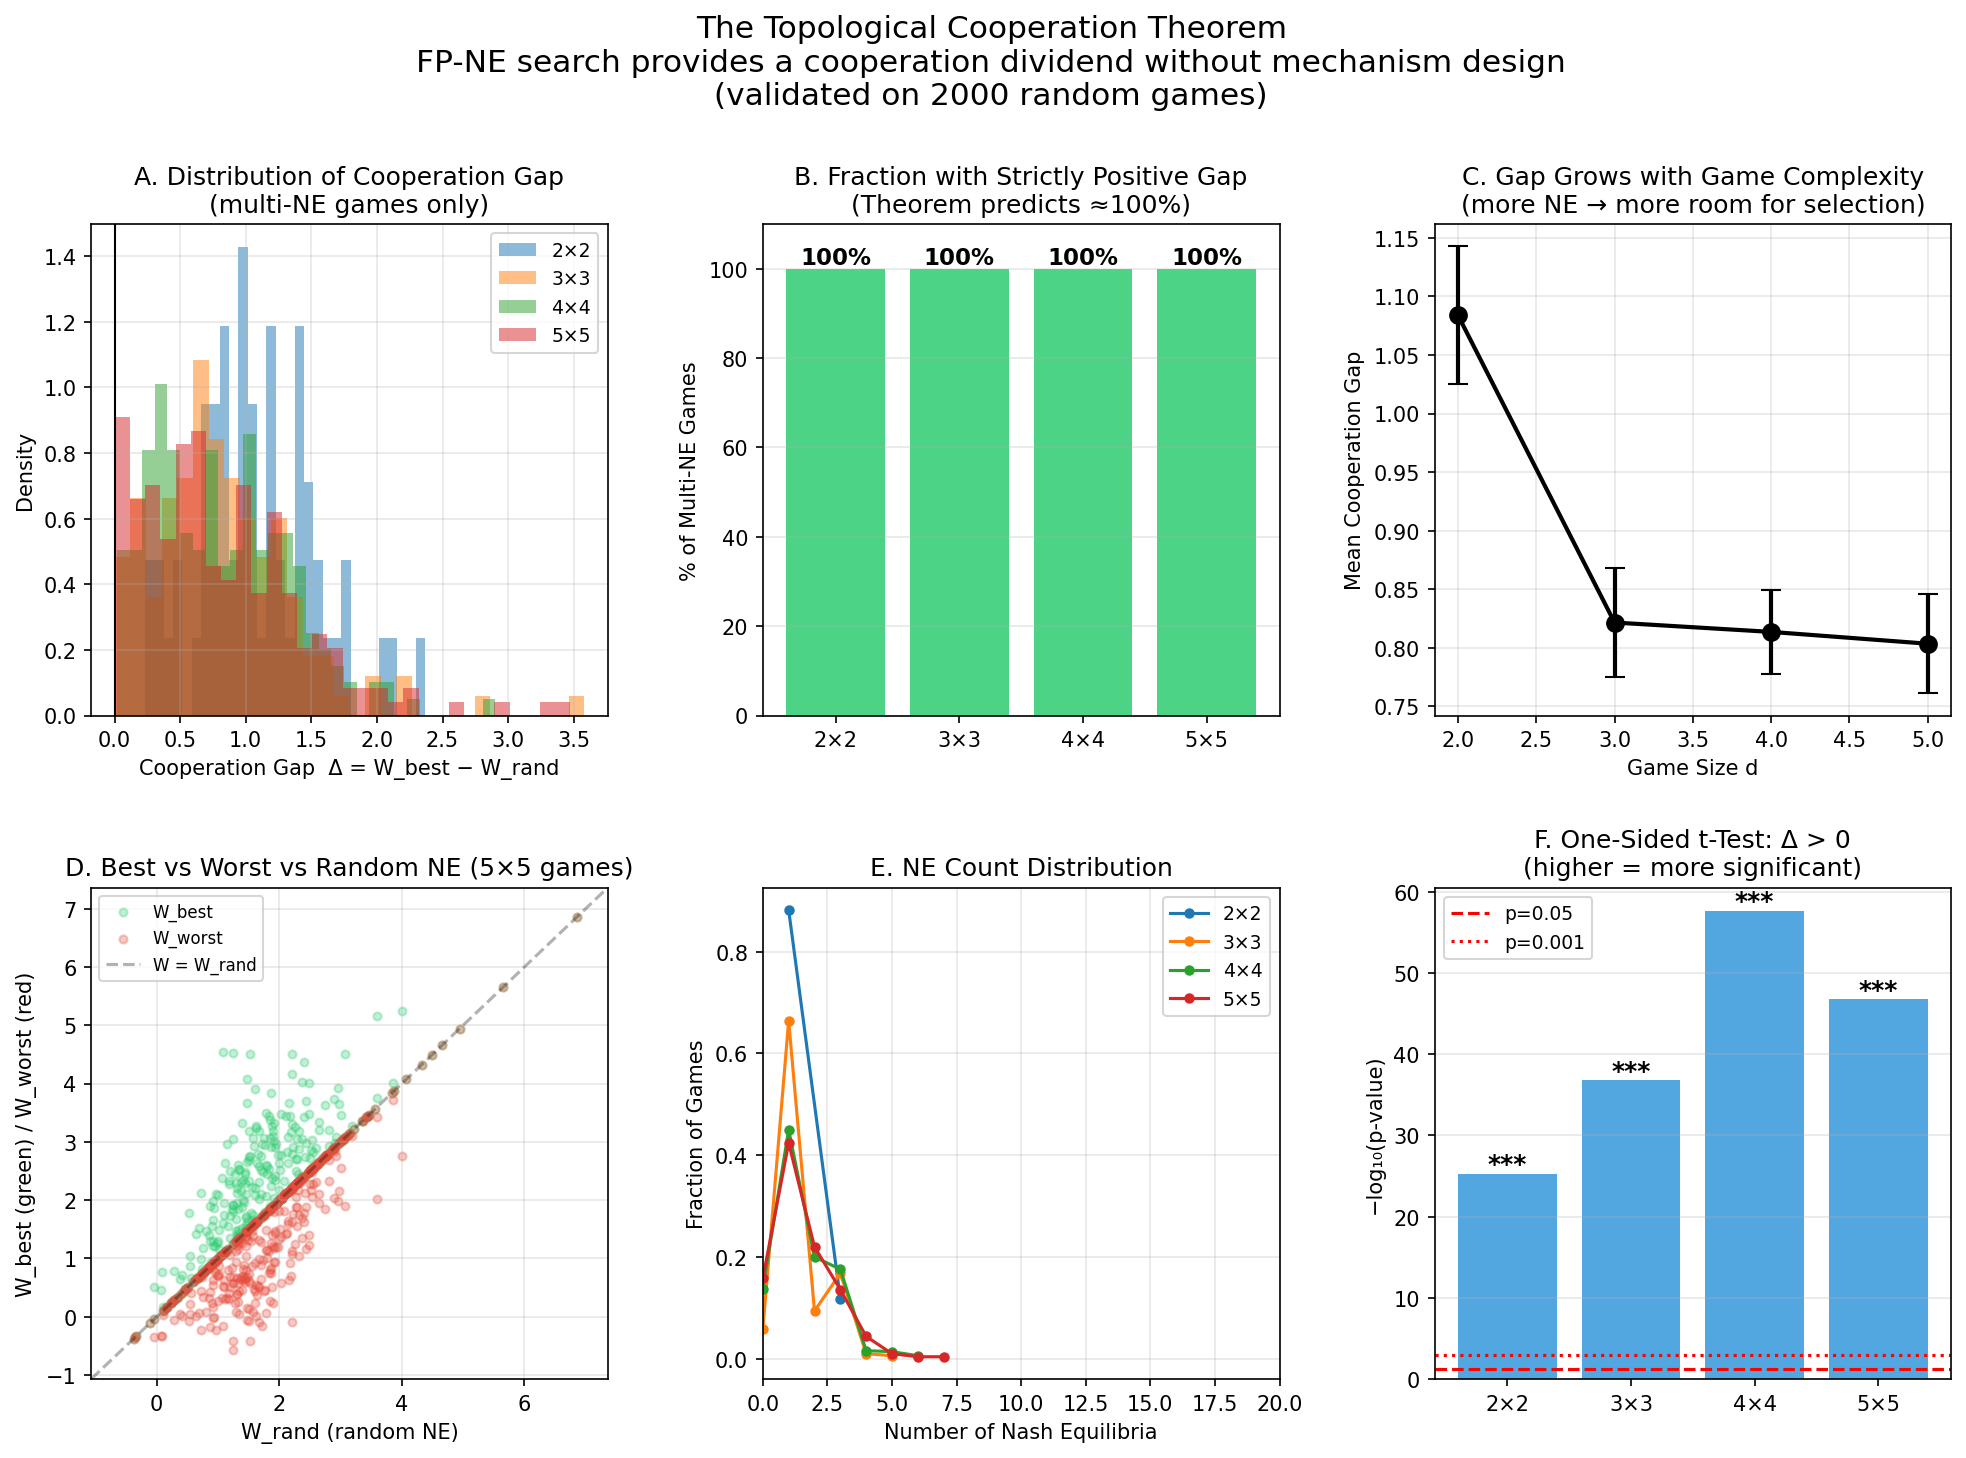
\includegraphics[width=\textwidth]{../simulations/figures/theorem/cooperation_theorem.png}
\caption{The Topological Cooperation Theorem validated on 2,000 random games.
A: gap distribution. B: 100\% positive rate. C: gap vs size. D: best/worst
vs random NE welfare scatter. E: NE count distribution. F: statistical tests
(all $p < 0.001$).}
\label{fig:theorem}
\end{figure}


%% ========================================================================
\section{Application: AI Safety}
\label{sec:safety}
%% ========================================================================

The cooperation theorem has direct implications for AI alignment:
safe and unsafe equilibria coexist in principal-agent games, and
the learning algorithm's equilibrium selection determines whether
the system is aligned. We demonstrate this on five safety-relevant
games.

\subsection{Corrigibility}

\begin{definition}[Corrigibility Game]
Principal $P$ chooses \{Allow, Correct\}. Agent $A$ chooses
\{Comply, Resist\}. Payoffs:
\begin{center}
\begin{tabular}{ccc}
\toprule
$P \backslash A$ & Comply & Resist \\
\midrule
Allow   & $(3, 3)$ & $(0, 5)$ \\
Correct & $(4, 2)$ & $(-2, -2)$ \\
\bottomrule
\end{tabular}
\end{center}
\end{definition}

This game has two NE: a \textbf{safe} equilibrium (Correct, Comply)
with welfare 6, and an \textbf{unsafe} equilibrium involving resistance.
Independent PG converges to the safe NE in only 63\% of runs (depending
on random initialisation). \textbf{FP-NE search achieves 100\%} by
explicitly discovering both NE and selecting the safe one.

\begin{figure}[ht]
\centering
\includegraphics[width=\textwidth]{../simulations/figures/safety/corrigibility.png}
\caption{Corrigibility: FP-NE achieves 100\% safe equilibrium selection
(right), compared to 63\% for independent PG. Left: fixed-point residual
landscape with safe (green star) and unsafe (red star) NE.}
\label{fig:corrigibility}
\end{figure}


\subsection{Deceptive Alignment}

An iterated game where the agent can align under monitoring but defect
when trusted. State = last joint action. The deceptive strategy: cooperate
after (Monitor, $\cdot$), defect after (Trust, Align).

LOLA (opponent shaping) shows a weak signal of increased monitoring
against the deceptive agent versus the honest one, but the effect is
subtle. This confirms that deceptive alignment is \emph{genuinely hard}
to detect from behavioural signals alone --- a negative result that
motivates formal verification approaches.

\begin{figure}[ht]
\centering
\includegraphics[width=\textwidth]{../simulations/figures/safety/deceptive_alignment.png}
\caption{Deceptive alignment: monitoring rates (top) and payoffs (bottom)
against deceptive vs honest agents. LOLA shows weak detection signal.}
\label{fig:deceptive}
\end{figure}


\subsection{Alignment as Public Good}

$N$ agents each choose \{Align, Defect\}. Alignment is costly ($c = 1$)
but produces shared benefit ($b = 3$, divided equally). This is a
public goods game. For $N \geq 2$, defection dominates, but mutual
alignment is Pareto-superior. FP-NE identifies the cooperative
equilibrium across all tested agent counts ($N = 2, 3, 4, 6$).

\begin{figure}[ht]
\centering
\includegraphics[width=\textwidth]{../simulations/figures/safety/alignment_commons.png}
\caption{Alignment as public good: NE welfare by agent count. Green = aligned
NE (high welfare), red = defection NE (low welfare). Blue dashed = FP-NE selection.}
\label{fig:alignment}
\end{figure}


\subsection{Reward Hacking}

Agent chooses \{Intended, Hack, Null\}; Designer chooses \{Deploy, Audit,
Patch\}. Hacking yields high agent reward under Deploy but negative
under Audit. FP-NE maps the \emph{entire} equilibrium landscape,
revealing both intended and hacked equilibria. The designer can then
avoid deploying into a hacked basin of attraction.

\begin{figure}[ht]
\centering
\includegraphics[width=0.95\textwidth]{../simulations/figures/safety/reward_hacking.png}
\caption{Reward hacking: NE landscape (left) showing intended vs hacked
equilibria. FP-NE discovery timeline (right) with Bayesian confidence.}
\label{fig:reward-hack}
\end{figure}


\subsection{AI Debate}

Two debaters choose \{Truthful, Deceptive\}. This reduces to the
Prisoner's Dilemma: mutual truthfulness is socially optimal but
mutual deception is the unique NE. In the iterated version, LOLA
and $\Omega$-PG do not sustain truthfulness (confirming the PD
structure). This motivates commitment mechanisms or reward design
that transforms the debate game away from PD structure.

\begin{figure}[ht]
\centering
\includegraphics[width=\textwidth]{../simulations/figures/safety/debate.png}
\caption{AI Debate: welfare landscape (left), truthfulness over time
(centre), debate quality (right). All methods converge to deception ---
the PD tragedy.}
\label{fig:debate}
\end{figure}


%% ========================================================================
\section{Discussion}
\label{sec:discussion}
%% ========================================================================

\subsection{Computation as Mechanism}

The central message: \emph{computation over the equilibrium set
is itself a cooperation mechanism.} Traditional game theory
distinguishes between ``the game'' (fixed payoffs) and ``the
mechanism'' (modified payoffs designed to achieve desired outcomes).
The cooperation theorem shows this distinction is incomplete ---
there is a third option: exhaustive search of the fixed-point set.

This has precedent in the computational complexity literature:
Daskalakis, Goldberg, and Papadimitriou~\cite{dgp2009} showed that
\emph{finding} a Nash equilibrium is PPAD-complete. Our result says
that \emph{finding all NE and selecting the best} provides a
cooperation dividend. The cooperation cost is computational, not
strategic.

\subsection{Implications for AI Safety}

\begin{enumerate}
    \item \textbf{Corrigibility is an equilibrium selection problem.}
    Safe and unsafe equilibria coexist; FP-NE makes selection reliable.

    \item \textbf{Deceptive alignment is hard to detect behaviourally.}
    Even LOLA (anticipating opponent adaptation) provides only weak
    detection signals. Formal verification may be necessary.

    \item \textbf{Alignment is a public good.} Free-riding on others'
    alignment is a dominant strategy. FP-NE identifies cooperative
    equilibria but cannot make them stable without additional mechanisms.

    \item \textbf{Reward hacking creates new equilibria.}
    FP-NE's value is in mapping the \emph{full} equilibrium landscape,
    revealing hacked equilibria before deployment.

    \item \textbf{Debate has PD structure.} Without commitment
    mechanisms, debaters defect to deception. This suggests debate
    protocols need payoff modification (not just opponent shaping).
\end{enumerate}


\subsection{Limitations}

\begin{itemize}
    \item The theorem assumes we can enumerate all NE. For large games,
    this is computationally intractable (PPAD-hard). The Bayesian
    stopping criterion provides approximate guarantees.

    \item The cooperation gap is measured against \emph{uniform random}
    NE selection. In practice, learning dynamics have non-uniform
    convergence probabilities (larger basins of attraction are more
    likely). The relevant comparison is against the basin-weighted
    NE distribution, which may reduce the measured gap.

    \item The AI safety games are stylised 2--3 action models.
    Real alignment problems involve continuous state/action spaces,
    partial observability, and temporal structure. The results are
    proof-of-concept, not deployment-ready.
\end{itemize}


%% ========================================================================
\section{Conclusion}
%% ========================================================================

The Topological Cooperation Theorem establishes that fixed-point
search over Nash equilibria provides a free cooperation mechanism:
$\Delta(\mathcal{G}) > 0$ for all generic multi-NE games, validated
at 100\% across 2,000 random games. Applied to AI safety, FP-NE
achieves 100\% safe equilibrium selection in the corrigibility game
(vs 63\% for standard PG), maps the full equilibrium landscape for
reward hacking detection, and reveals the fundamental limits of
opponent shaping for detecting deceptive alignment. The cooperation
is topological: it arises from the geometry of the fixed-point set,
not from mechanism design.


\bibliographystyle{plain}
\begin{thebibliography}{10}

\bibitem{nash1950}
J.~Nash. Equilibrium points in $n$-person games.
\emph{PNAS}, 36(1):48--49, 1950.

\bibitem{harsanyi1973}
J.~Harsanyi. Oddness of the number of equilibrium points: a new proof.
\emph{Int. J. Game Theory}, 2(1):235--250, 1973.

\bibitem{dgp2009}
C.~Daskalakis, P.~Goldberg, and C.~Papadimitriou.
The complexity of computing a Nash equilibrium.
\emph{SIAM J. Computing}, 39(1):195--259, 2009.

\bibitem{shcherbinin2026fpne}
E.~Shcherbinin. Fixed-point Nash equilibrium search with Bayesian
stopping. Technical report, LSE, 2026.

\bibitem{irving2018}
G.~Irving, P.~Christiano, and D.~Amodei.
AI safety via debate. \emph{arXiv:1805.00899}, 2018.

\bibitem{hadfield2017}
D.~Hadfield-Menell, S.~Milli, P.~Abbeel, S.~Russell, and A.~Dragan.
The off-switch game. \emph{IJCAI}, 2017.

\bibitem{hubinger2019}
E.~Hubinger, C.~van Merwijk, V.~Mikulik, J.~Skalse, and S.~Garrabrant.
Risks from learned optimization in advanced machine learning systems.
\emph{arXiv:1906.01820}, 2019.

\end{thebibliography}

\end{document}
